\section{Vorbereitungsfragen}
\subsection{Wie ist die hydraulische Leistung definiert?}
%
\begin{equation}
	P_{ Eigenverbrauch }= U_{ LR} \cdot I_{ LR }\cdot \dot Q = \dot m * g* H
\label{eq:2}
\end{equation}
%
\subsection{Skizzieren Sie den typischen Verlauf einer Rohrleitungskennlinie}
%
\begin{figure}[!ht]
		\centering
		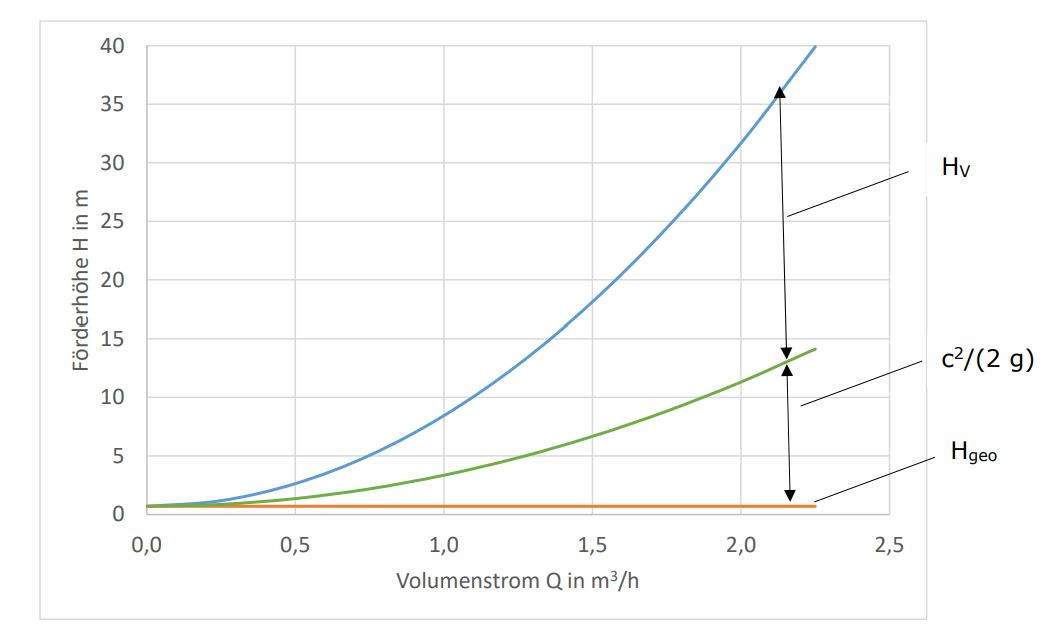
\includegraphics[width=0.5\textwidth]{Abbildungen/Rohrleitungskennlinie}
		\caption{Rohrleitungskennlinie bei vollständig geöfneter Düse}
		\label{fig:230512_Rohrleitungskennlinie}
\end{figure}
%
\subsection{Welche Proportionalität ergib sich bei Strömungsmaschinen zwischen Leistung und Drehzahl?}
Die Leistung $P$ ist wie folgt definiert.
%
\begin{equation}
	P= M*2*\pi*n
\label{eq:230512_MechanischeLeistung}
\end{equation}
%
Dabei ist $n$ die Drezahl und $M$ das Moment.
\subsection{Wie lässt sich der Betriebspunkt einer Pelton-Turbine einstellen?}
Der Betriebspunkt ist mit dem Volumenstrom/Strahldurchmesser,durch eine angelegte Last am Generator oder den Erregerstrom $I_{Err}$steuerbar. Dabei ist der optimale Betriebspunkt über die optimale Drehzahl zu finden. Dabei liegt die optimale Drehzahl bei der halben Austrittsgeschwindigkeit aus der Düse.

\subsection{Welcher hydraulische Parameter wird zur Regelung der Pelton-Turbine verändert?
Durch welche Einstellung passiert das?}
Die Düsennadel kann so eingestellt werden, dass der Durchflussquerschnitt sich verändert. Mit dem Durchflussquerschnitt lässt sich dann der Volumenstrom Q steuern und somit die Drehzahl der Perlton Turbine.